% ==========================================
% BAB IV DESAIN KONSEP SOLUSI
% ==========================================
\chapter{DESAIN KONSEP SOLUSI}
\label{chap:desain-konsep-solusi}

\section{Model Konseptual Solusi yang Diusulkan}
Berdasarkan analisis masalah dan pemilihan solusi pada bab sebelumnya, penelitian ini mengusulkan arsitektur sistem hibrida yang mengintegrasikan \textit{Machine Learning} (ML), \textit{Explainable Artificial Intelligence} (XAI), dan \textit{Large Language Model} (LLM) berbasis \textit{Retrieval-Augmented Generation} (RAG).

Gambar \ref{fig:konsep-solusi} mengilustrasikan desain konsep solusi (\textit{proposed system}) yang dirancang untuk mengubah data klinis pasien menjadi prediksi risiko yang akurat, transparan, dan mudah dipahami.

\begin{figure}[h]
    \centering
    % Pastikan nama file tidak menggunakan spasi. Gunakan underscore atau dash.
    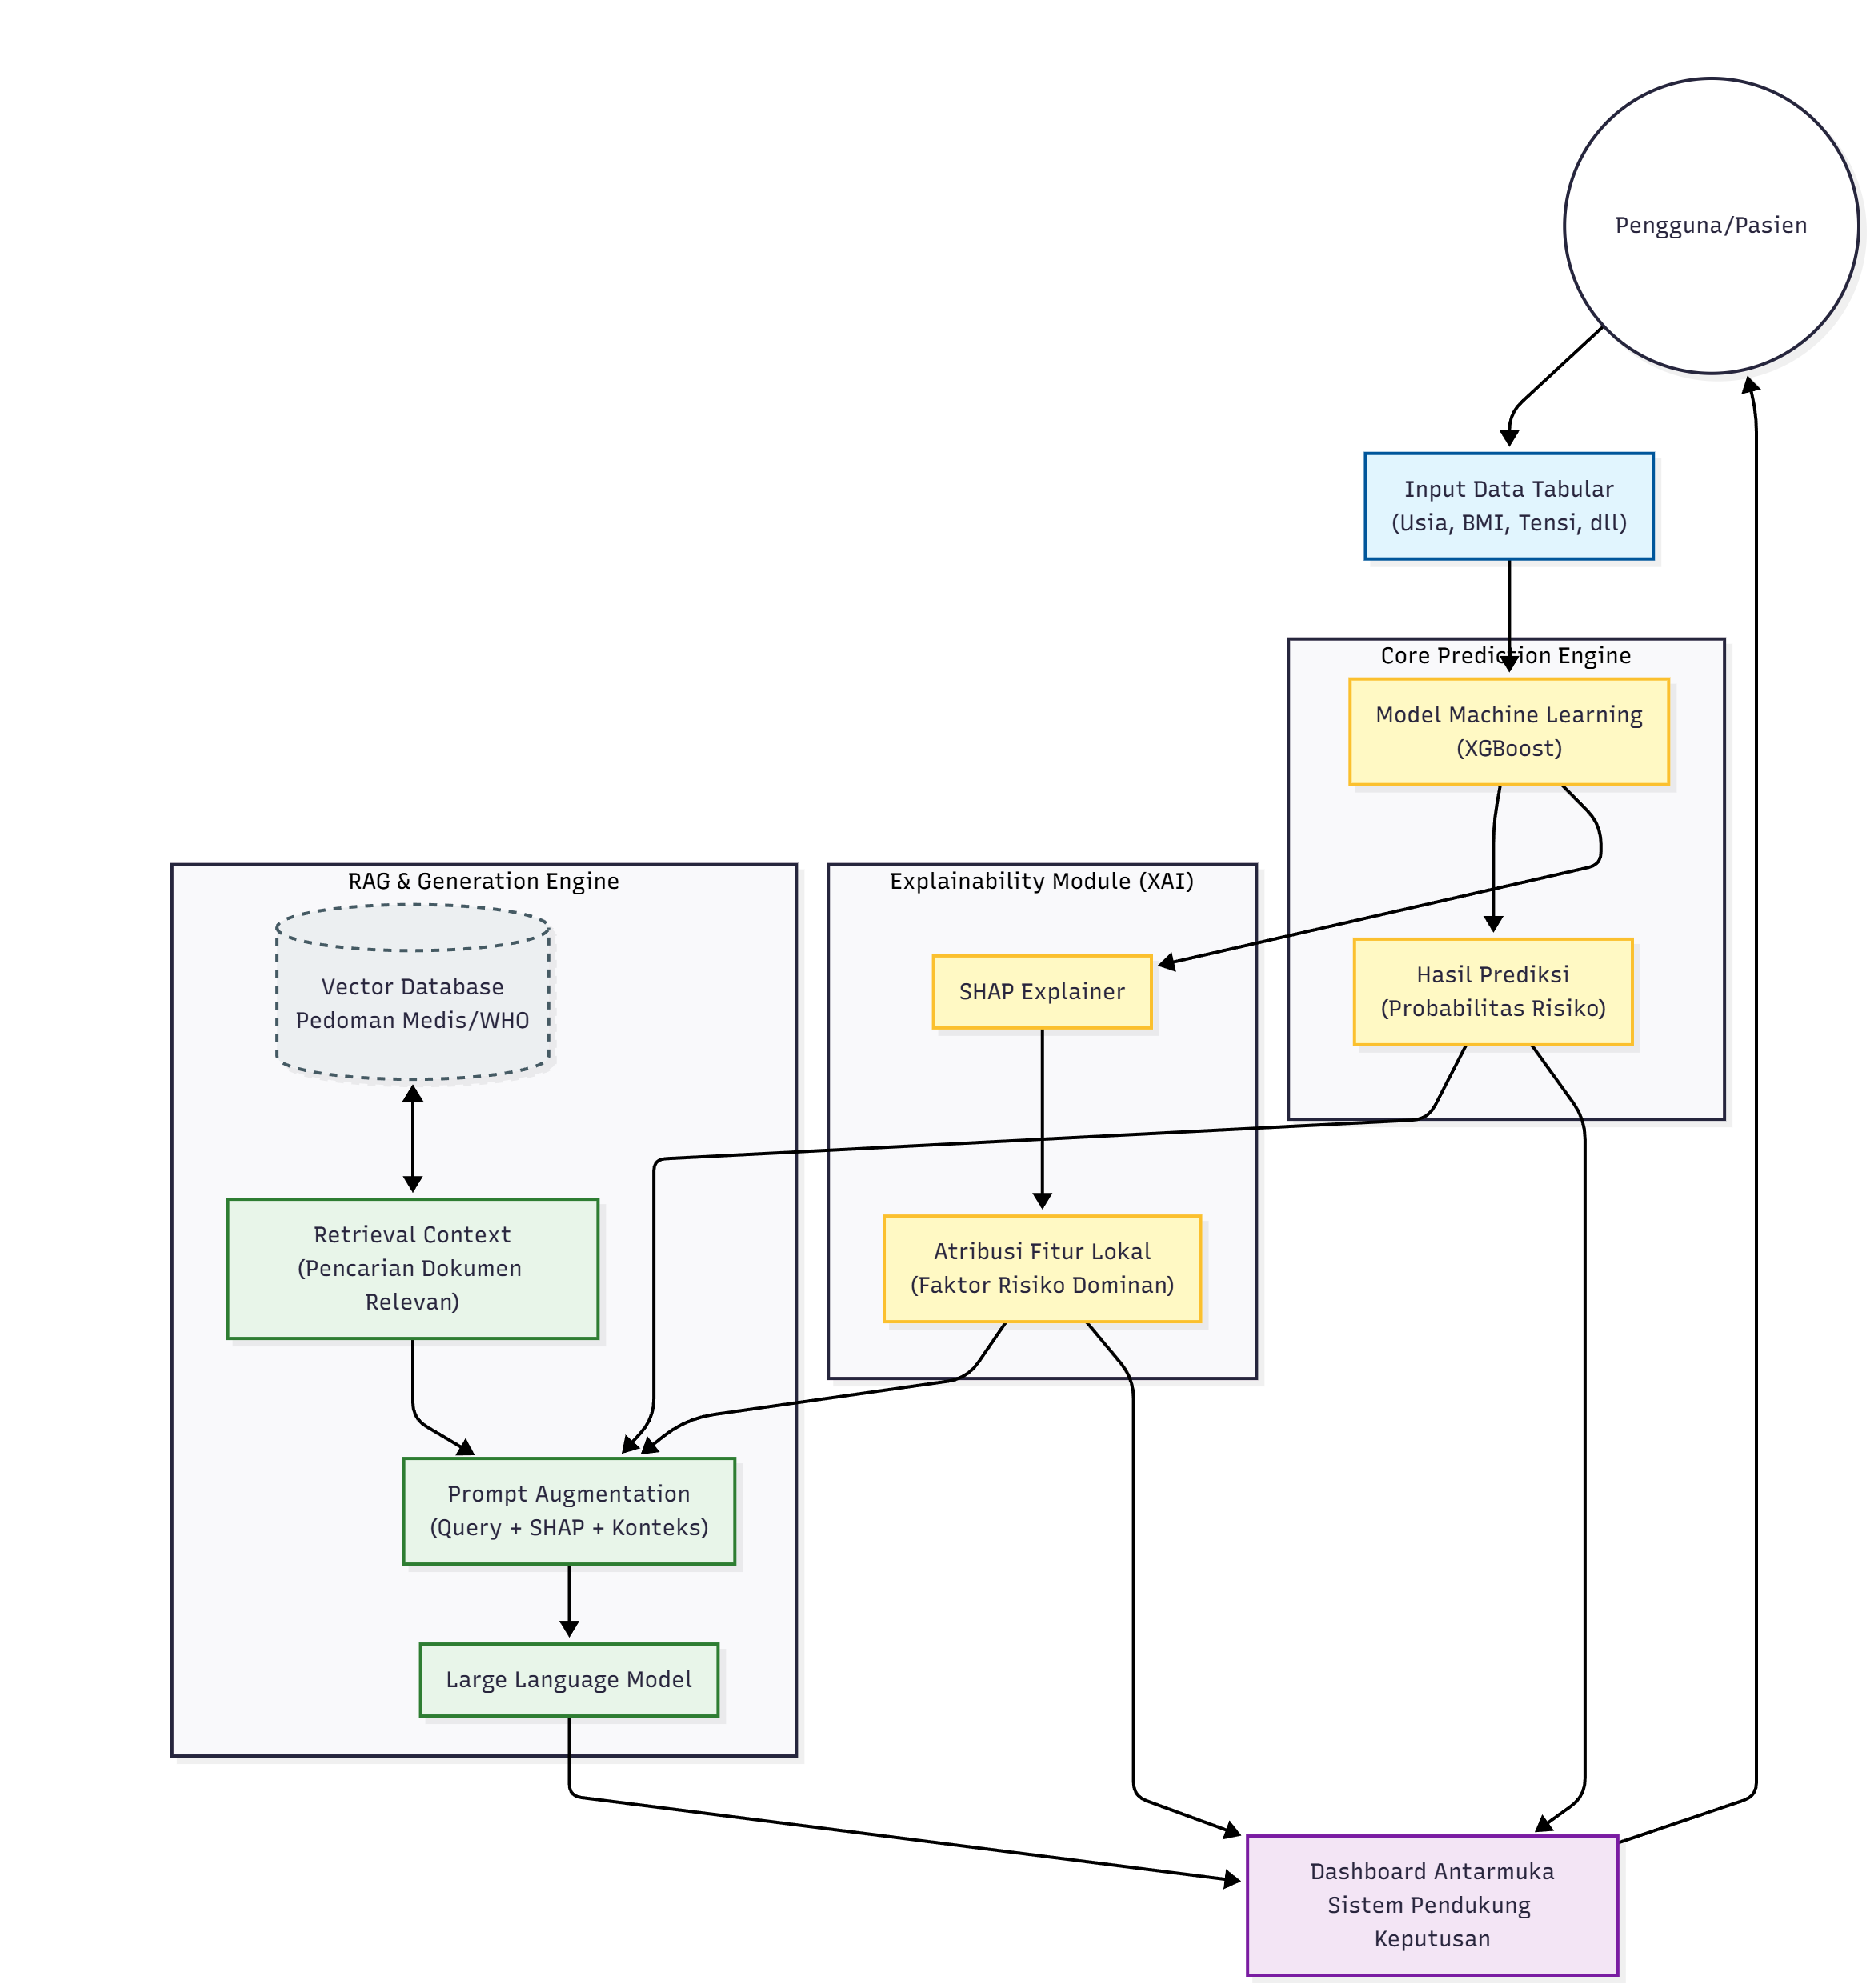
\includegraphics[width=0.8\textwidth]{image/Desain Konsep Solusi Sistem.png} 
    \caption{Desain Konsep Solusi Sistem}
    \label{fig:konsep-solusi}
\end{figure}

\subsection{Penjelasan Alur Kerja Sistem}
Sistem yang diusulkan bekerja dalam alur sekuensial otomatis sebagai berikut:

\begin{enumerate}
    \item Pengguna memasukkan parameter kesehatan (seperti usia, tekanan darah, IMT, dan riwayat keluarga) ke dalam sistem.
    
    \item Model ML (XGBoost) memproses data tersebut untuk menghasilkan skor probabilitas risiko hipertensi (misalnya: 56\% Berisiko).
    
    \item Secara paralel, modul XAI menggunakan metode SHAP untuk membedah \textit{black box} model ML. Modul ini mengidentifikasi variabel mana yang paling berkontribusi terhadap skor risiko tersebut, misalnya tinggi konsumsi garam dan IMT, yang menjadi kontributor utama.
    
    \item Sistem mengambil hasil atribusi fitur dari SHAP. Lalu setelahnya, sistem melakukan pencarian (\textit{retrieval}) pada basis data vektor yang berisi pedoman medis yang relevan dengan faktor risiko yang ditemukan, seperti pedoman dari Kemenkes atau WHO. LLM akan menggabungkan hasil prediksi, alasan dari SHAP, dan referensi medis untuk menyusun narasi penjelasan yang personal dan valid.
    
    \item Pengguna menerima tiga luaran terintegrasi: Status Risiko (ML), Grafik Faktor Penyebab (XAI), dan Penjelasan Naratif serta Saran Medis (RAG-LLM).
\end{enumerate}

\subsection{Arsitektur Sistem}
Setelah merancang alur kerja operasional sistem yang baru, langkah krusial berikutnya adalah menerjemahkan kebutuhan fungsional tersebut ke dalam spesifikasi teknis yang konkret. Diagram arsitektur sistem diperlukan untuk memetakan bagaimana komponen perangkat lunak, aliran data, dan infrastruktur saling berinteraksi guna menjalankan logika prediksi secara stabil, aman, dan skalabel.

Gambar \ref{fig:arsitektur-teknis} berikut mengilustrasikan arsitektur teknis sistem yang dirancang dengan pendekatan berbasis layanan (\textit{service-based architecture}).

\begin{figure}[h]
    \centering
    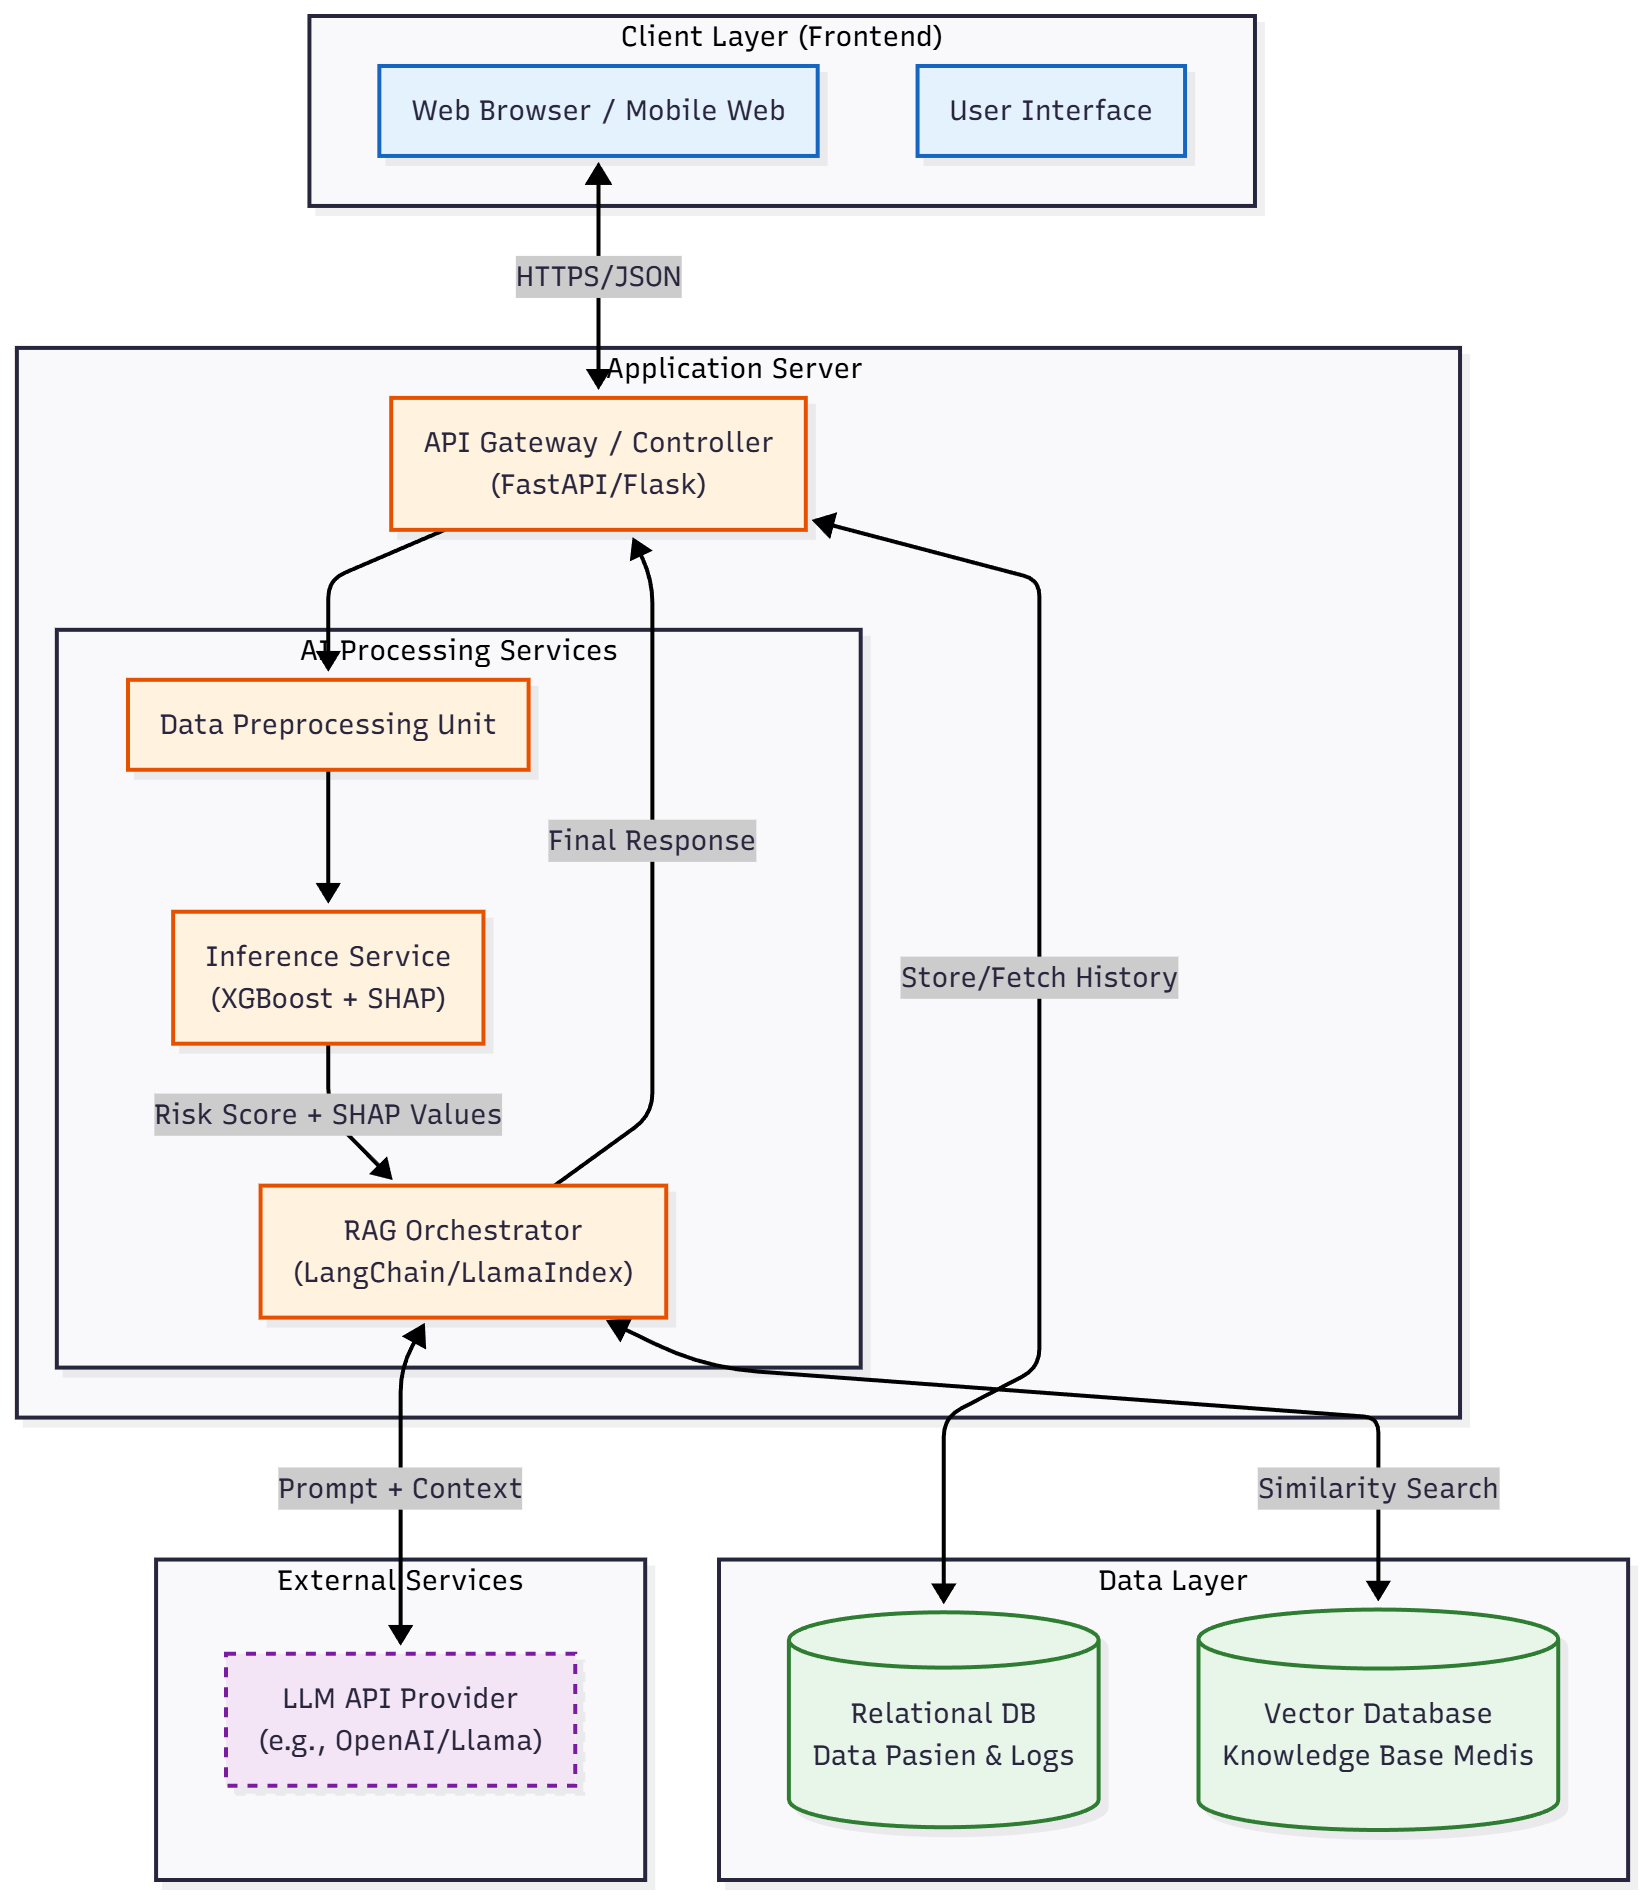
\includegraphics[width=0.8\textwidth]{image/arsitektur sistem.png}
    \caption{Arsitektur Teknis Sistem }
    \label{fig:arsitektur-teknis}
\end{figure}

Berdasarkan Gambar \ref{fig:arsitektur-teknis} di atas, sistem terbagi menjadi empat lapisan utama dengan fungsi spesifik sebagai berikut:

\begin{itemize}
    \item Client Layer (Frontend) \\
    Lapisan ini merupakan titik interaksi pengguna, baik melalui peramban web desktop maupun perangkat seluler. Lapisan ini bertugas menangkap input data klinis pasien dan memvisualisasikan hasil prediksi berupa grafik risiko dan narasi penjelasan yang dikirimkan oleh server melalui protokol HTTPS/JSON yang aman.

    \item Application Layer \\
    Lapisan ini berfungsi sebagai otak pemrosesan sistem. Lapisan ini terdiri dari API Gateway yang mengatur lalu lintas data, serta unit AI Processing Services yang menjalankan tiga fungsi sekuensial:
    \begin{enumerate}
        \item \textit{Data Preprocessing} untuk membersihkan input.
        \item \textit{Inference Service} yang menjalankan model XGBoost dan SHAP untuk menghitung skor risiko.
        \item \textit{RAG Orchestrator} yang meramu \textit{prompt} untuk model bahasa.
    \end{enumerate}

    \item Data Layer \\
    Lapisan ini bertanggung jawab atas persistensi data dengan menggunakan dua jenis basis data. \textit{Relational Database} digunakan untuk menyimpan data terstruktur pasien dan log riwayat prediksi, sedangkan \textit{vector database} digunakan khusus untuk menyimpan \textit{embedding} dokumen pedoman medis yang memungkinkan pencarian konteks semantik (\textit{similarity search}) yang cepat.

    \item External Services \\
    Sistem terhubung dengan penyedia layanan \textit{Large Language Model} (LLM) pihak ketiga seperti OpenAI atau model \textit{open-source} terhosting lainnya. Komponen ini menerima \textit{prompt} yang telah diperkaya dengan konteks medis dari sistem internal untuk menghasilkan narasi penjelasan yang natural, namun tetap tervalidasi.
\end{itemize}

\section{Perbandingan dengan Sistem Saat Ini}
Desain konsep solusi di atas menawarkan perubahan paradigma dari pendekatan konvensional yang digambarkan pada Bab III menjadi pendekatan berbasis kecerdasan buatan yang terintegrasi. Perbandingan komparatif antara kondisi saat ini (\textit{As-Is}) dan solusi yang diusulkan (\textit{To-Be}) dirangkum dalam Gambar \ref{fig:alur-diagnosis}.

% \begin{table}[htbp]
%     \centering
%     \caption{Perbandingan Sistem Konvensional vs Sistem Usulan}
%     \label{tab:perbandingan-sistem}
%     \renewcommand{\arraystretch}{1.5} % Menambah jarak antar baris agar lebih rapi
%     \begin{tabular}{|p{3.5cm}|p{5.5cm}|p{5.5cm}|}
%     \hline
%     \textbf{Aspek Pembanding} & \textbf{Sistem Saat Ini (As-Is)} & \textbf{Solusi Usulan (To-Be)} \\
%     \hline
%     Pendekatan Diagnosis & 
%     Reaktif \& Manual. Diagnosis bergantung pada pengukuran sesaat di klinik dan ingatan dokter terhadap pedoman. & 
%     Prediktif \& Otomatis. Sistem memprediksi risiko secara dini berdasarkan pola data historis menggunakan \textit{Machine Learning}. \\
%     \hline
%     Transparansi Keputusan & 
%     Intuitif/Implisit. Keputusan dokter didasarkan pada \textit{tacit knowledge} yang sulit dijelaskan secara kuantitatif kepada pasien. & 
%     \textit{Explainable} (XAI). Sistem menyediakan visualisasi atribusi fitur (SHAP) yang menunjukkan secara persis variabel penyebab risiko secara matematis. \\
%     \hline
%     Penyampaian Informasi & 
%     Lisan \& Terbatas. Penjelasan risiko sering kali singkat karena keterbatasan waktu konsultasi, menyebabkan pasien kurang paham. & 
%     Narasi Personal (GenAI). LLM menghasilkan penjelasan tertulis yang disesuaikan dengan profil pasien, menjabarkan hubungan sebab-akibat dengan bahasa alami. \\
%     \hline
%     Validitas Referensi & 
%     Variatif. Sangat bergantung pada \textit{update} pengetahuan tenaga medis masing-masing. & 
%     Terstandarisasi (RAG). Setiap saran yang dihasilkan divalidasi silang (\textit{cross-reference}) dengan dokumen pedoman medis terkini di \textit{Vector Database}. \\
%     \hline
%     Alur Kerja & 
%     Linear dan membutuhkan eskalasi manual bertingkat (perawat $\rightarrow$ dokter). & 
%     Terintegrasi dan \textit{real-time}, memberikan \textit{second opinion} instan sebelum eskalasi ke ahli. \\
%     \hline
%     \end{tabular}
% \end{table}

\begin{figure}[H]
    \centering
    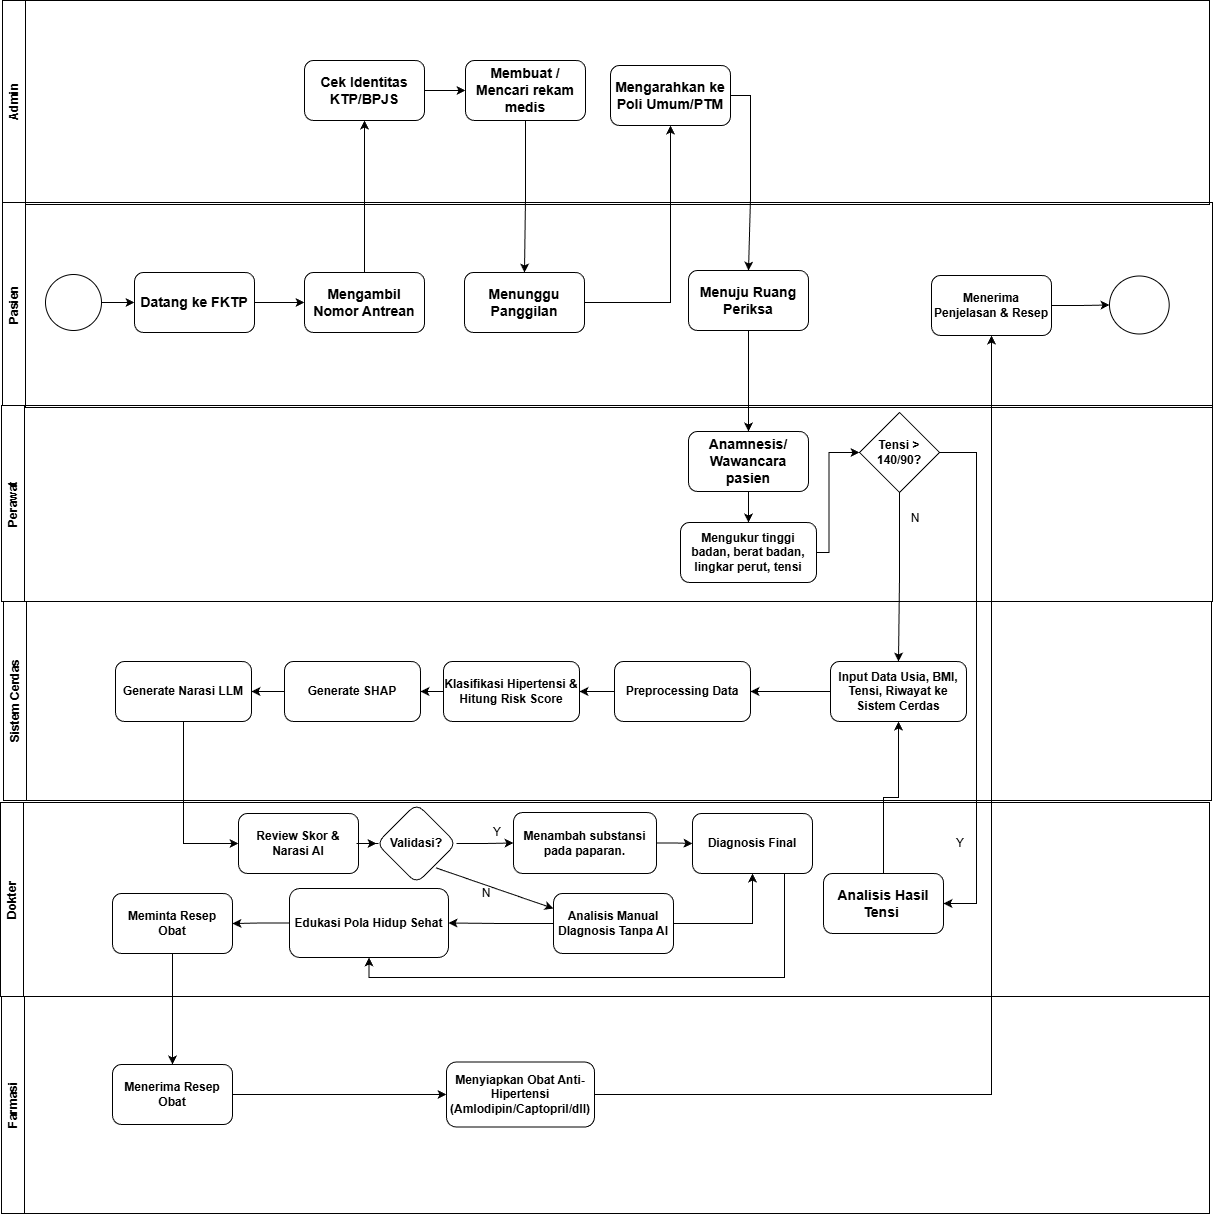
\includegraphics[width=0.8\textwidth]{image/alursistemtobe.png}
    \caption{Alur Diagnosis Hipertensi di Fasilitas Kesehatan Tingkat Pertama (FKTP) (To-Be)}
    \label{fig:alur-diagnosis}
\end{figure}

Secara visual, jika dibandingkan dengan kondisi awal, desain usulan menggambarkan adanya otomatisasi dalam proses penalaran klinis. Pada tahap ini, dokter tidak lagi melakukan observasi data pasien secara manual, melainkan memasukkan data tersebut ke dalam sistem yang berfungsi sebagai pendukung dalam pengambilan keputusan.

Meskipun demikian, penekanan utama tetap berada pada peran dokter sebagai pengambil keputusan akhir. Informasi maupun rekomendasi yang diberikan sistem harus dipahami, ditafsirkan, dan dievaluasi kembali oleh dokter untuk memperoleh wawasan klinis yang komprehensif. Dengan demikian, sistem ini dirancang bukan untuk menggantikan fungsi dokter dalam menentukan keputusan medis, tetapi untuk mengurangi beban kognitif dalam proses analisis data sehingga dokter dapat membuat keputusan yang lebih tepat, efisien, dan berbasis informasi.